
\begin{figure}[!ht]
\begin{center}
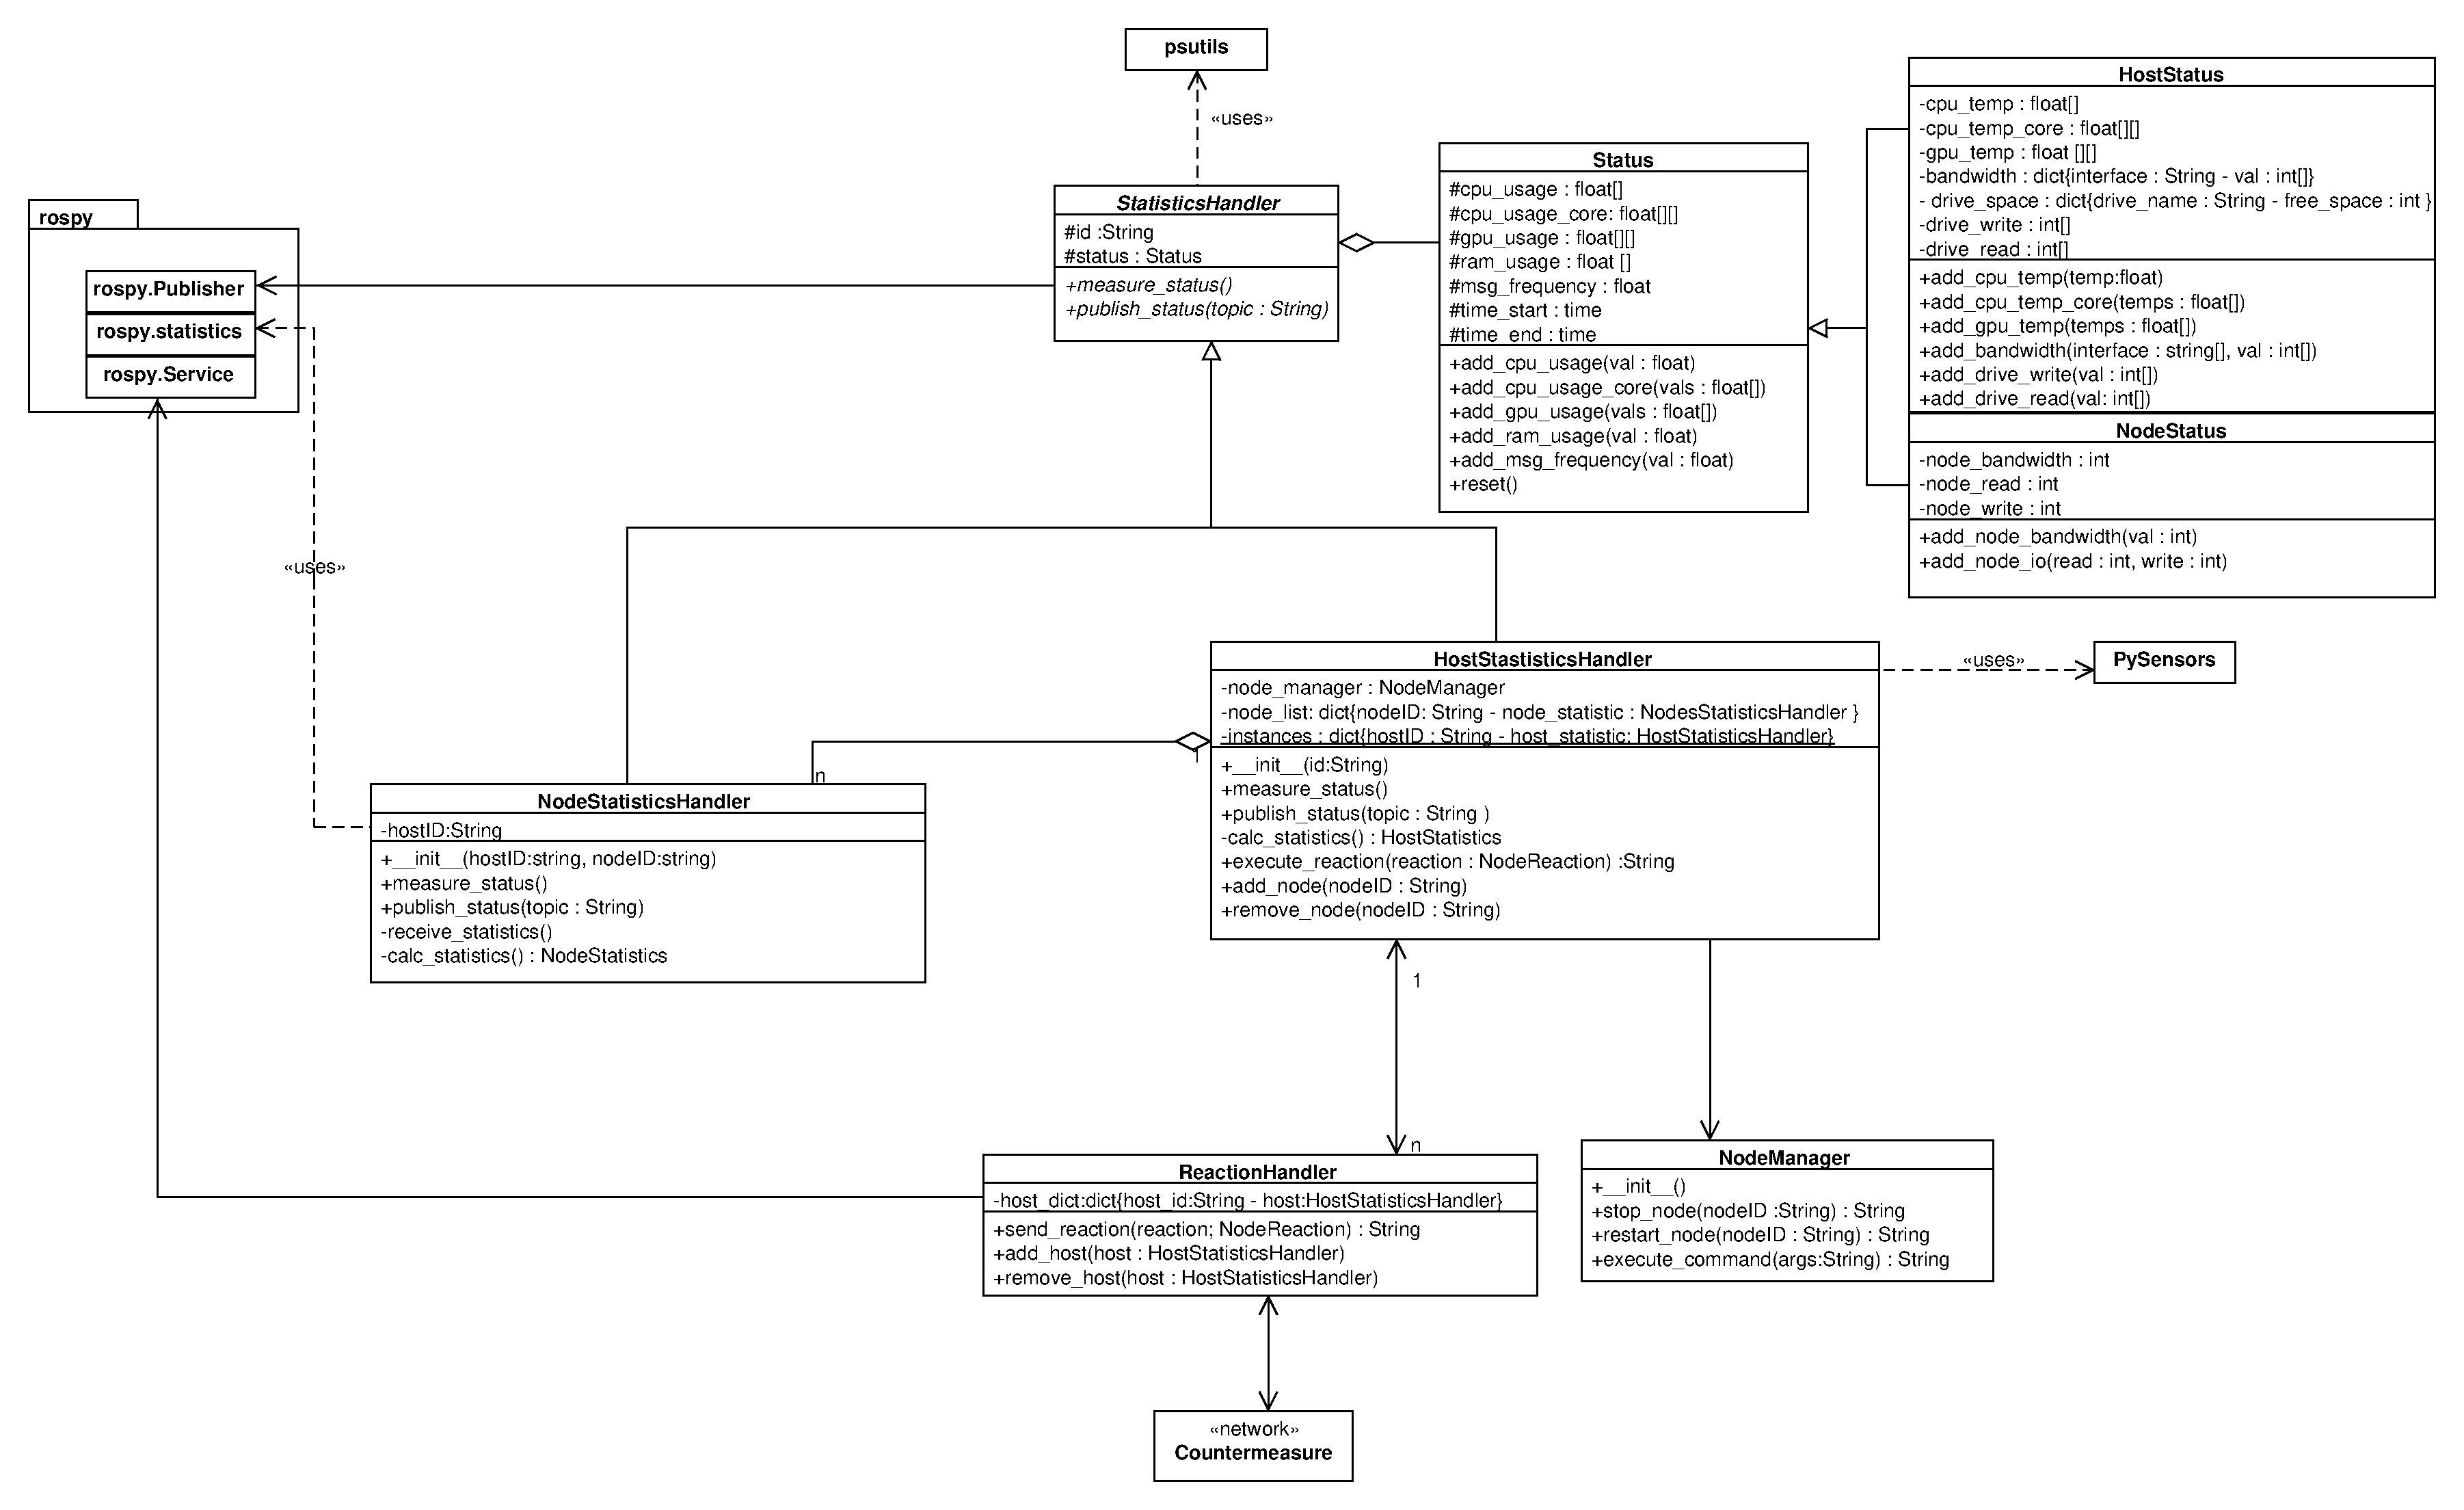
\includegraphics[width = 1.0 \linewidth]{./diagram_pictures/NodeInterface/erfassung.pdf}
\caption{UML diagram of the NodeInterface package}
\end{center}
\end{figure}
\newpage


\subsection{StatisticsHandler}
\begin{figure}[htbp]
	\begin{minipage}[t]{7cm}
		\vspace{0pt}
		\centering
		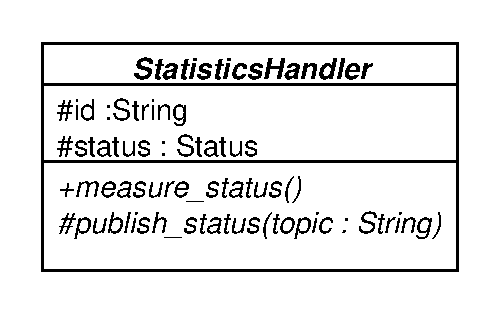
\includegraphics[scale=0.6]{./diagram_pictures/NodeInterface/StatisticsHandler.pdf}
	\end{minipage}
	\hfill
	\begin{minipage}[t]{8cm}
		\vspace{10pt}
		Abstract Class to Handle Statistics of Hosts or Nodes.
	\end{minipage}
\end{figure}



\subsubsection{Attributes}
\begin{itemize}
	\item \textbf{protected String id}\\
	Id of the Host or Node.	
	\item \textbf{protected Status status}\\
	Holds the current status.
\end{itemize}

\subsubsection{Methods}
\begin{itemize}
\item \textbf{public void measure\_status()}\\
			Collects information about the current status using psutils.
			Triggered periodically.
\item \textbf{public void publish\_status(String topic)}\\
			Publishes the current status to a topic using ROS's publisher-subscriber mechanism.
\end{itemize}



\subsection{HostStatisticsHandler}
\begin{figure}[htbp]
	\begin{minipage}[t]{7cm}
		\vspace{0pt}
		\centering
		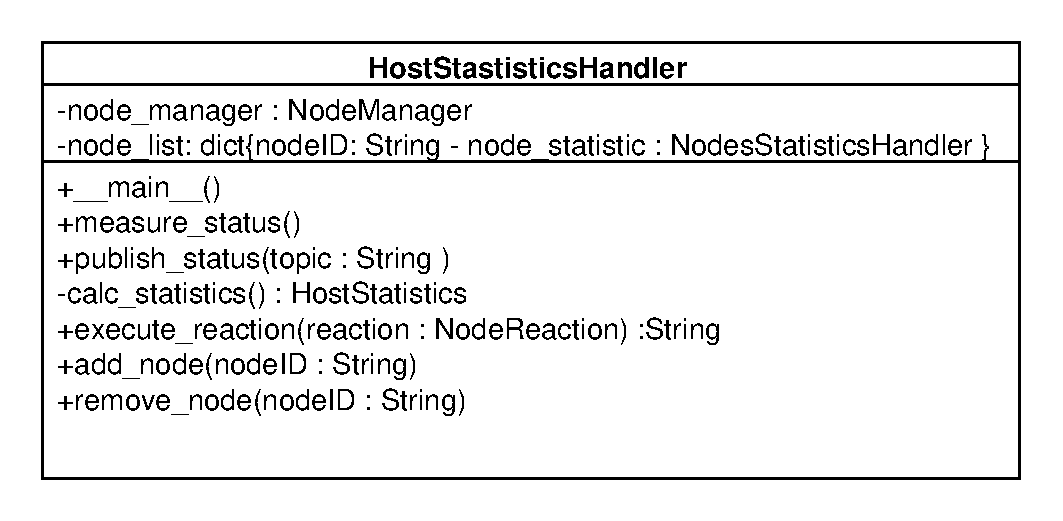
\includegraphics[scale=0.6]{./diagram_pictures/NodeInterface/HostStatisticsHandler.pdf}
	\end{minipage}
	\hfill
	\begin{minipage}[t]{5cm}
		\vspace{10pt}
		Represents a host , limited to one instance per host. Collects statistics about the current state of the host and sends them using the 				publisher-subscriber mechanism.
	\end{minipage}
\end{figure}


\subsubsection{Attributes}
\begin{itemize}
	\item \textbf{private NodeManager node\_manager}\\
			NodeManager providing function to restart and stop Nodes.
	\item \textbf{private  dict\{String nodeID  - NodesStatisticsHandler node\_statistic  \} node\_list}\\
			Dictionary holding all Nodes and their statistics, currently running on the host.
\end{itemize}

\subsubsection{Methods}
\begin{itemize}
	\item \textbf{public void measure\_status()}\\
			Collects information about the host's current status using psutils.
			Triggered periodically.
	\item \textbf{public void publish\_status(String topic)}\\
			Publishes the current status to a topic using ROS's publisher-subscriber mechanism.
			Triggered periodically.
	\item \textbf{public String execute\_reaction(NodeReaction reaction)}\\
			Parses through the reaction and calls the appropriate method from the NodeManager. Uses ROS Services.
			Returns a message about operation's success.
	\item \textbf{public void add\_node(String nodeID)}\\
			Adds a Node with the given id to the host.
	\item \textbf{public void remove\_node(String nodeID)}\\
			Removes the Node with the given id from the host.
	\item \textbf{private HostStatistics calc\_statistics}\\
			Calculates statistics like mean, standard deviation and max from the status.
			Returns an instance of HostStatistics which can be published.
\end{itemize}

\subsection{NodeStatisticsHandler}
\begin{figure}[htbp]
	\begin{minipage}[t]{7cm}
		\vspace{0pt}
		\centering
		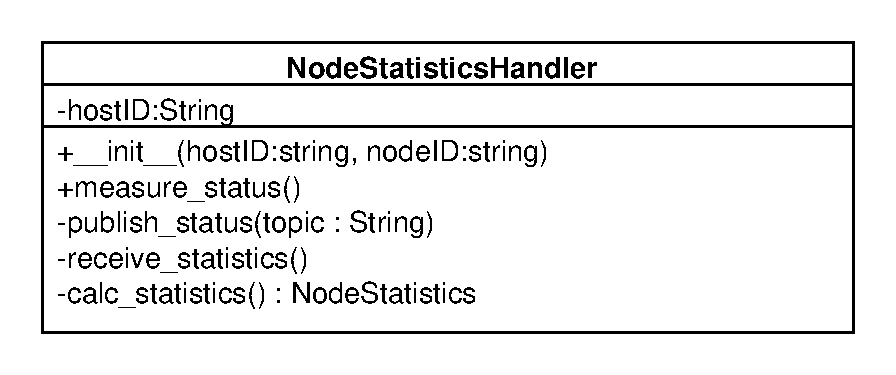
\includegraphics[scale=0.6]{./diagram_pictures/NodeInterface/NodeStatisticsHandler.pdf}
	\end{minipage}
	\hfill
	\begin{minipage}[t]{6cm}
		\vspace{10pt}
		Holds the statistics of an individual Node.
	\end{minipage}
\end{figure}


\subsubsection{Attributes}
\begin{itemize}
	\item \textbf{private String hostID}\\
	Id of the host this node runs on.
\end{itemize}

\subsubsection{Methods}
\begin{itemize}
	\item \textbf{public void measure\_status()}\\
	Collects information about the node's current status using psutils and rospy.statistics
	Triggered periodically.
	\item \textbf{public void publish\_status()}\\
	Publishes the current status to a topic using ROS's publisher-subscriber mechanism.
	Triggered periodically.
	\item \textbf{private void receive\_statistics()}\\
	Receives the statistics published by ROS Topic statistics
	\item \textbf{private NodeStatistic calc\_statistics}\\
	Calculates statistics like mean, standard deviation and max from the status.
	Returns an instance of NodeStatistic which can be published.
\end{itemize}

\subsection{Status}
\begin{figure}[htbp]
	\begin{minipage}[t]{7cm}
		\vspace{0pt}
		\centering
		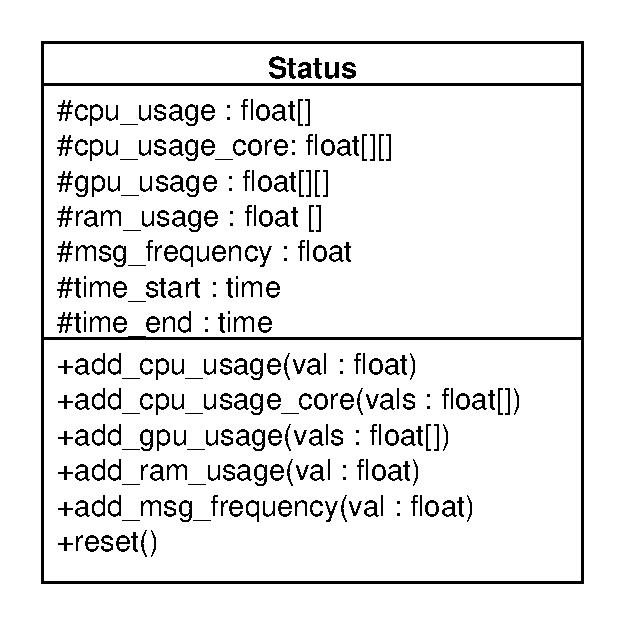
\includegraphics[scale=0.6]{./diagram_pictures/NodeInterface/Status.pdf}
	\end{minipage}
	\hfill
	\begin{minipage}[t]{8cm}
		\vspace{10pt}
		Container Class to Store information about the current status.
	\end{minipage}
\end{figure}


\subsubsection{Attributes}
\begin{itemize}
	\item \textbf{protected float[] cpu\_usage }\\
	Percentage of the cpu used.
	\item \textbf{protected float[][] cpu\_usage\_core}\\
	Percentage of the cpu used per core.
	\item \textbf{protected float[] ram\_usage}\\
	Percentage of ram used.
	\item \textbf{protected time time\_start}\\
	Time of the start of the measurements.
	\item \textbf{protected time time\_end}\\
	Time of the end of the measurements.
\end{itemize}

\subsubsection{Methods}
\begin{itemize}
	\item \textbf{public void add\_cpu\_usage(float value}\\
	Adds another measured value to cpu\_usage.
	\item \textbf{public void add\_cpu\_usage\_core(float[] values)}\\
	Adds another measured value to per core cpu\_usage\_core.
	\item \textbf{public void add\_gpu\_usage(float[] values}\\
	Adds another measured value per card to gpu\_usage.
	\item \textbf{public void add\_ram\_usage(float value)}\\
	Adds another measured value to ram\_usage.
	\item \textbf{public void reset()}\\
	Resets the status.
\end{itemize}

\subsection{HostStatus}

\begin{figure}[htbp]
	\begin{minipage}[t]{7cm}
		\vspace{0pt}
		\centering
		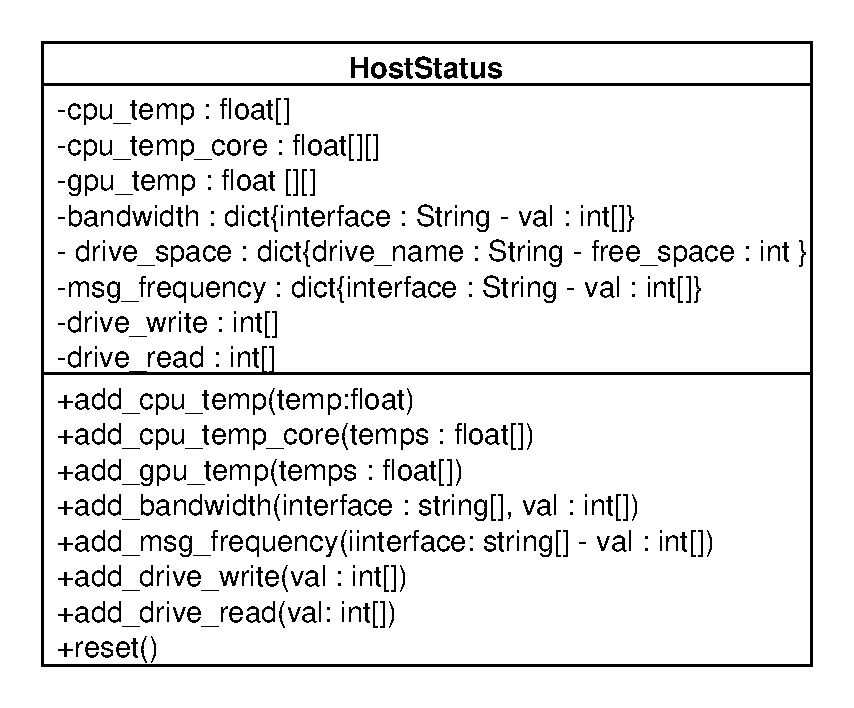
\includegraphics[scale=0.6]{./diagram_pictures/NodeInterface/HostStatus.pdf}
	\end{minipage}
	\hfill
	\begin{minipage}[t]{7cm}
		\vspace{10pt}
		Extension of Status , to store additional information used by hosts.
	\end{minipage}
\end{figure}


\subsubsection{Attributes}
\begin{itemize}
	\item \textbf{private float[] cpu\_temp}\\
	Current CPU temperature in Celsius.
	\item \textbf{private float[][] cpu\_temp\_core}\\
	Current CPU temperature per core in Celsius.
	\item \textbf{private float[][] gpu\_temp\_core}\\
	Current GPU temperature per GPU in Celsius.
	\item \textbf{private dict\{String interface - int[] bytes\} bandwidth }\\
	Bytes sent through a NIC since the start of the time window.
	\item \textbf{private dict\{String interface - int[] msg\_freq\} msg\_frequency}\\
	Frequency of network calls by NIC.
	\item \textbf{private dict\{String drive - int[] free\_space\} bandwidth}\\
	Free Space per drive.
	\item \textbf{private int[][] drive\_write}\\
	Bytes written per drive since the start of the time window.
	\item \textbf{private int[][] drive\_read}\\
	Bytes read per drive since the start of the time window.
\end{itemize}

\subsubsection{Methods}
\begin{itemize}
	\item \textbf{public void add\_cpu\_temp(float temp)}\\
	Adds another measured value to cpu\_temp.
	\item \textbf{public void add\_cpu\_temp\_core(float[] temps)}\\
	Adds another measured value per core to cpu\_temp\_core.
	\item \textbf{public void add\_gpu\_temp(float[] temps)}\\
	Adds another measured value per card to gpu\_temp.
	\item \textbf{public void add\_bandwidth(String[] Interface, int[] bandwidth)}\\
	Adds another measured value to bandwidth.
	\item \textbf{public void add\_msg\_freq(String[] Interface, int[] msg\_freq)}\\
	Adds another measured value to msg\_frequency.
	\item \textbf{public void add\_drive\_write(int[] byte)}\\
	Adds another measured value per drive to drive\_write.
	\item \textbf{public void add\_drive\_read(int[] byte)}\\
	Adds another measured value per drive to drive\_read.
	\item \textbf{reset()}\\
	Resets the status.
\end{itemize}

\subsection{NodeStatus}
\begin{figure}[htbp]
	\begin{minipage}[t]{7cm}
		\vspace{0pt}
		\centering
		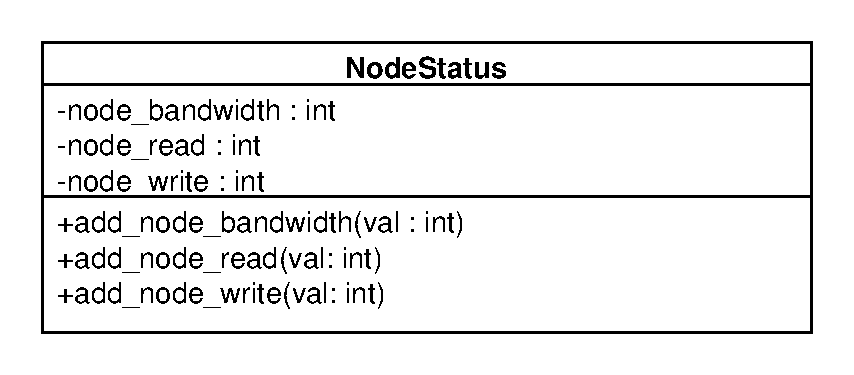
\includegraphics[scale=0.6]{./diagram_pictures/NodeInterface/NodeStatus.pdf}
	\end{minipage}
	\hfill
	\begin{minipage}[t]{7cm}
		\vspace{10pt}
		Extension of Status , to store additional information used by nodes.
	\end{minipage}
\end{figure}


\subsubsection{Attributes}
\begin{itemize}
	\item \textbf{private int[] node\_bandwidth}\\
	Bytes the node has sent through the network.
	\item \textbf{private int[] node\_read}\\
	Bytes the node has read from a hard drive since the start of the time window.
	\item \textbf{private int[] node\_write}\\
	Bytes the node has written to a hard drive since the start of the time window.
	\item \textbf{private int[] node\_msg\_frequency}\\
	Frequency of networks calls done by node.
\end{itemize}

\subsubsection{Methods}
\begin{itemize}
	\item \textbf{public void add\_node\_bandwidth(int byte)}\\
	Adds another measured value  to node\_bandwidth.
	\item \textbf{public void add\_node\_io(int read, int write)}\\
	Adds another pair of measured read and write values to node\_read and node\_write.
	\item \textbf{reset()}\\
	Resets the status.
\end{itemize}

\subsection{NodeManager}
\begin{figure}[htbp]
	\begin{minipage}[t]{7cm}
		\vspace{0pt}
		\centering
		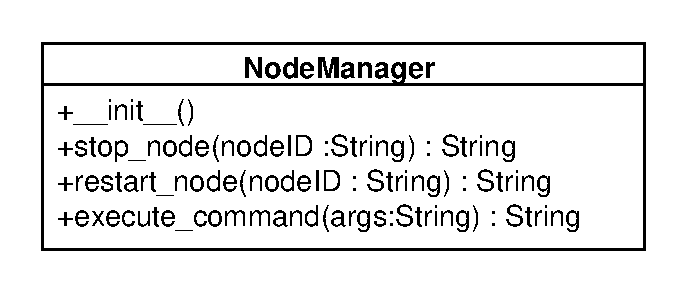
\includegraphics[scale=0.6]{./diagram_pictures/NodeInterface/NodeManager.pdf}
	\end{minipage}
	\hfill
	\begin{minipage}[t]{8cm}
		\vspace{10pt}
		Can restart or stop nodes or execute a countermeasure.
	\end{minipage}
\end{figure}


\subsubsection{Methods}
\begin{itemize}
	\item \textbf{public String stop\_node(String nodeID)}\\
	Stops the node with the given id.
	Returns a message about operation's success.
	\item \textbf{public String restart\_node(String nodeID)}\\
	Restarts a node with the given id.
	Returns a message about operation's success.
	\item \textbf{public String execute\_command(String[] args)}\\
	Executes a system call with the given arguments.
	Returns a message about operation's success.
\end{itemize}


\subsection{psutils}
Library to acquire the system's usage statistics. For a more in-depth documentation, see the official psutils documentation.

\subsubsection{Used methods}
\begin{itemize}
	\item \textbf{psutil.cpu\_percent(interval, boolean percpu)}\\
	Return a float representing the current system-wide CPU usage.
	\item \textbf{psutil.virtual\_memory()}\\
	Return statistics about system memory usage.
	\item \textbf{psutil.net\_io\_counters(boolean pernic)}\\
	Return system-wide network I/O statistics.
	\item \textbf{psutil.disk\_usage(String path)}\\
	Return disk usage statistics about the given path.
	\item \textbf{psutil.disk\_io\_counters(boolean perdisk)}
	Return system-wide disk I/O statistics.
	\item \textbf{psutil.disk\_partitions()}\\
	Return all mounted disk partitions as a list of namedtuples.
	\item \textbf{psutil.Process(pid )}\\
	Represents an  process with the given pid
\end{itemize}


	